\documentclass[11pt,a4paper]{article}

%===========================
% Packages
%===========================
\usepackage[utf8]{inputenc}
\usepackage[T1]{fontenc}
\usepackage{geometry}
\geometry{margin=1in}
\usepackage{amsmath,amssymb,amsthm}
\usepackage{bm}
\usepackage{xcolor}
\usepackage{graphicx}
\usepackage{hyperref}
\usepackage{authblk}

\newcommand{\red}[1]{\textcolor{red}{#1}}

\hypersetup{
  colorlinks=true,
  linkcolor=blue,
  citecolor=blue,
  urlcolor=blue
}

%===========================
% Title / Author
%===========================
\title{\textbf{The Enchan Field:}\\
An Effective Field Framework for Geometric Stabilization and Non-Linear Relaxation}

\author[1]{Mitsuhiro Kobayashi}
\affil[1]{Tokyo, Japan\\
\texttt{enchan.theory@gmail.com}}

\date{\today}

%===========================
% Document
%===========================
\begin{document}

\maketitle

\begin{abstract}
The Enchan Field is proposed as an effective field framework for describing geometric stabilization across continuous and discrete systems. Its starting point is the possibility that gravity-like stabilization phenomena are not governed solely by material source terms, but also by the relaxation structure of geometry itself. In this view, coherent large-scale structures arise from a field medium whose response becomes non-linear when deformation, concentration, or interaction intensity exceeds a characteristic scale.

This paper introduces the Enchan Field as a geometric order field $S(x)$, formulates its effective relaxation equation, and interprets its non-linear screening response as finite field tension rather than as an externally imposed correction. The same stabilization principle is then translated into discrete graph dynamics, where high-degree hub nodes act as localized over-concentrations of interaction intensity. Under purely linear aggregation, these hubs can dominate the relaxation landscape and cause premature convergence. Under Enchan Field screening, excessive local concentration is regularized, allowing the system to relax toward stable phase boundaries that correspond to candidate graph cuts.

The computational engine known as Enchan Cosmic is therefore interpreted here not as the theoretical starting point, but as a discrete realization of the Enchan Field principle. Empirical observations on scale-free networks suggest that finite-tension relaxation can suppress hub-induced collapse while preserving deterministic reproducibility. The result is a unified proposal: geometric stabilization in continuous fields and deterministic optimization in discrete topologies can be described as manifestations of non-linear relaxation within an interaction medium.
\end{abstract}

\tableofcontents

\clearpage

\section{Introduction}

Gravity is usually described through the distribution of material sources. The geometric formulation of gravitation, however, suggests a deeper starting point: the observed dynamics of a system may reflect not only what is present as matter, but also how geometry itself relaxes, stabilizes, and resists deformation.

The Enchan Field is proposed as an effective field framework for this geometric stabilization. Rather than beginning from an additional substance or from a pre-existing modified-dynamics model, this paper begins from a simpler question: can the stabilizing effect inferred from large-scale coherent structures be represented as a property of the interaction field itself?

In the Enchan interpretation, geometry is not treated as a passive background. It is modeled as a medium with an order parameter, a relaxation law, and a finite capacity to absorb concentration. When interaction intensity remains within ordinary bounds, the field may appear approximately linear. When concentration becomes excessive, however, the field enters a non-linear response regime. This finite-tension response prevents unbounded distortion and produces stabilization.

This paper develops the Enchan Field before introducing its computational realization. This is important because Enchan Cosmic, described elsewhere as a deterministic graph dynamics engine, is not the theoretical premise of the present work. It is a discrete realization of the broader field principle: optimization on a graph can be interpreted as geometric relaxation within a constrained interaction medium.

Historically, the computational implementation was developed after the Enchan Field notes had already been written and publicly released \cite{KobayashiFieldNotes}. Its original purpose was not to build a graph solver, but to test whether the field equations and relaxation principles described in those notes could be instantiated as a working computational process. Only afterward did the implementation reveal solver-like behavior and a connection to graph optimization.

An earlier technical note, titled \emph{The Enchan Field Equation}, formulated the Enchan Field using a standard scalar-field Lagrangian. That precursor emphasized fluctuation-driven spatial order, the fixed-point relation between a primordial fluctuation field $F$ and an emergent order field $S$, and the formation of stable geometric defects. The present paper should be read as a generalization of that earlier formulation: the standard linear kinetic term is replaced by a non-linear finite-tension kinetic vessel, and the Enchan Field is reframed as an effective geometric stabilization field rather than as a model whose primary subject is any particular inferred matter sector.

The main contributions of this paper are:
\begin{itemize}
    \item the formulation of the Enchan Field as an effective geometric stabilization field;
    \item the generalization of the earlier scalar-field Enchan Field Equation into a non-linear finite-tension kinetic framework;
    \item the interpretation of non-linear screening as finite field tension and over-concentration regularization;
    \item the translation of continuous field relaxation into discrete graph dynamics;
    \item the identification of hub-induced collapse as a form of topological over-curvature;
    \item the interpretation of deterministic graph optimization as phase-boundary formation in a relaxed interaction field.
\end{itemize}

\clearpage

\section{What Is the Enchan Field?}

The Enchan Field is an effective interaction field whose scalar order parameter $S(x)$ represents the stabilized geometric configuration of a system. It is not introduced as a new material component. It is introduced as a way to describe how geometry-like structure can converge toward stable configurations under fluctuation, concentration, and constraint.

The central idea is that a system may contain not only local interactions, but also a global relaxation medium through which those interactions become organized. In ordinary descriptions, interaction is often treated as pairwise coupling between objects. In the Enchan Field view, such pairwise interactions are embedded in a continuous medium whose deformation determines the global stabilization path.

Thus, $S(x)$ should be read as a geometric order parameter. High values, gradients, or curvature in $S$ indicate regions where the interaction medium is deformed. Stable configurations correspond to relaxed states in which the field has absorbed or redistributed local fluctuation without entering runaway distortion.

\subsection{Field, Geometry, and Stabilization}

The Enchan Field is motivated by a geometric view of gravity-like phenomena. If gravity is interpreted not merely as a force transmitted between material bodies, but as an expression of geometric structure, then stabilization may also be understood geometrically. A coherent structure can persist because the underlying interaction geometry relaxes into a stable configuration.

This perspective shifts the question from ``what additional substance produces the observed stabilization?'' to ``what geometric response of the field produces the observed stabilization?'' The Enchan Field is the proposed mathematical object used to describe that response.

\subsection{Relation to the Earlier Enchan Field Equation}

The earlier Enchan Field Equation introduced the axiomatic relation
\[
F = \partial_t \epsilon, \qquad S = \operatorname{Fix}(F),
\]
where a microscopic fluctuation process gives rise to an emergent stabilized order field. In that formulation, $S$ was modeled with a standard quadratic kinetic term and a potential $V(S)$ responsible for stability, vacuum selection, and topological defect formation.

The present work preserves the conceptual core of that formulation---space-like order is driven by fluctuation and stabilized through field dynamics---but changes the mathematical status of the kinetic sector. The quadratic kinetic term is now interpreted as the weak-concentration limit of a more general non-linear response. This allows finite field tension, screening, and over-concentration regularization to arise from the field equation itself, rather than being appended as an external damping rule.

\subsection{Finite Field Tension}

A key postulate of the Enchan Field is finite field tension. A continuous interaction medium cannot sustain unlimited concentration while remaining linear. Beyond a characteristic scale, the effective interaction law must change. The change is not arbitrary damping; it is the field's own resistance to unbounded deformation.

This principle is later expressed computationally as a non-linear screening factor. In the field interpretation, however, screening is not an external patch. It is the mathematical signature of a medium whose response saturates when local concentration exceeds its stable range.

\clearpage

\section{Effective Field Formulation}

In the Enchan framework, emergent spatial order $S$ is modeled as a stabilized fixed point of a fluctuation field $F$. The field $F$ represents structural pressure, source fluctuation, or interaction imbalance. The field $S$ represents the resulting geometric order after relaxation.

\subsection{From the linear precursor to finite-tension dynamics}

The earlier scalar-field formulation used the standard kinetic structure
\begin{equation}
\mathcal{L}_{\rm precursor}
= \frac{1}{2}(\partial_\mu S)(\partial^\mu S) + FS - V(S).
\end{equation}
This expression is retained as the weak-field or weak-concentration approximation. It is sufficient for deriving the basic fluctuation--stabilization relation, but it does not by itself encode the finite-tension principle: under extreme gradients, the quadratic kinetic term continues to scale without changing its response law.

The present formulation therefore replaces the quadratic kinetic term with a non-linear kinetic vessel. This is the central mathematical upgrade from the earlier Enchan Field Equation to the present v1.0.0 formulation.

\subsection{Field Variables and Interpretation}

To formalize this mechanism, we first define the core variables of the effective field:
\begin{itemize}
    \item \textbf{Geometric Order Field $S(x)$ [Dimensionless]:} The order parameter representing the local state of geometric relaxation or time dilation. High gradients in $S$ correspond to strong interaction intensity or spatial curvature.
    \item \textbf{Fluctuation Source $F(x)$:} The external driving force, structural pressure, or primordial interaction imbalance that pushes the system away from an empty configuration.
    \item \textbf{Stabilizing Potential $V(S)$:} The self-interaction energy of the field. This term is responsible for vacuum selection, anchoring, and the formation of stable phase boundaries (topological defects).
\end{itemize}

\subsection{Lagrangian formulation and finite field tension}
A linear field assumes that the interaction medium can sustain infinite concentration without changing its elastic properties. To model a physical saturation limit---finite field tension---we introduce a non-linear kinetic term (a $k$-essence type formulation). 

We define the kinetic invariant:
\begin{equation}
\mathcal{X} \equiv \frac{\nabla_\mu S\,\nabla^\mu S}{a_0^2}
\end{equation}
where $a_0$ is the characteristic saturation scale of the field. The effective Enchan Field $S(x)$ is then governed by the following Lagrangian density:
\begin{equation}
\mathcal{L} \;=\;
\mathcal{K}(\mathcal{X})
\;+\; F S
\;-\; V(S)
\label{eq:Lagrangian}
\end{equation}
where $\mathcal{K}(\mathcal{X})$ is a non-linear kinetic function that reduces to the standard linear form ($\mathcal{K}(\mathcal{X}) \propto \mathcal{X}$) in the weak-field limit, but saturates when the local concentration $\mathcal{X}$ becomes large. $F$ acts as a source term, and $V(S)$ is a self-interaction potential governing stability and defect formation.

This formulation directly embeds the geometric stabilization into the fundamental dynamics of the field, rather than treating it as a post-hoc correction.

\subsection{Euler--Lagrange equation of motion}
Varying Eq.~\eqref{eq:Lagrangian} with respect to $S$ yields the generalized Euler--Lagrange equation:
\begin{equation}
\nabla_\mu \left( \frac{\partial \mathcal{K}}{\partial \mathcal{X}} \nabla^\mu S \right) \;=\; F \;-\; \frac{\partial V}{\partial S}
\label{eq:FieldEq}
\end{equation}
If we define the effective response function as $\mu(\mathcal{X}) \equiv \frac{\partial \mathcal{K}}{\partial \mathcal{X}}$, the field equation becomes:
\begin{equation}
\nabla_\mu \Big( \mu(\mathcal{X}) \nabla^\mu S \Big) \;=\; F \;-\; \frac{\partial V}{\partial S}
\label{eq:FieldEqMu}
\end{equation}

This equation explicitly demonstrates how the field's finite tension modifies its own propagation. In regions of extreme concentration, $\mu(\mathcal{X})$ deviates from unity, dampening the effective coupling and preventing the field from diverging. In this sense, convergence is not an external optimization instruction; it is the field's own relaxation mechanism derived directly from first principles.

\clearpage

\section{Non-Linear Stabilization and Screening}

A linear field response assumes that interaction intensity can be extrapolated without bound. The Enchan Field rejects this unrestricted extrapolation. When local concentration becomes too large, the field enters a non-linear regime and reduces the effective propagation of excessive influence.

Let $D$ denote a local measure of interaction intensity or field deformation. The Enchan Field introduces a characteristic scale $a_0$ beyond which the linear approximation ceases to be valid. A simple screening response can be written as
\begin{equation}
\mu(D) \approx \frac{1}{1 + (|D|/a_0)^\alpha},
\end{equation}
where $a_0$ is the saturation threshold and $\alpha$ controls the sharpness of attenuation.

For $|D| \ll a_0$, the field behaves approximately linearly. For $|D| \gg a_0$, the effective interaction is attenuated. This is the mathematical expression of finite field tension: the medium does not permit a localized concentration to dominate the global relaxation process without resistance.

\clearpage

\section{Astrophysical Interpretation}

The Enchan Field was motivated by the suspicion that gravity-like stabilization may be more fundamentally geometric than material. In large-scale systems, observed coherence and persistent rotation profiles suggest that geometry may possess its own stabilizing response.

In astrophysical applications, time derivatives are considered negligible for the background configuration of $S$, simplifying the relation to $\square S \approx -\nabla^2 S$. Assuming a potential $V(S)$ that supports stabilized textures or topological defects, an asymptotic solution at radius $r$ may take a logarithmic form:
\begin{equation}
S(r) \sim \eta \ln\left(\frac{r}{r_c}\right),
\end{equation}
where $\eta$ and $r_c$ are constants.

Defining the interaction field intensity as $D(r) = \|\nabla S\|$, we obtain:
\begin{equation}
D(r) \sim \frac{\eta}{r}.
\end{equation}
The corresponding energy density scales as $\rho(r) \propto 1/r^2$. In a Newtonian approximation, the enclosed effective mass profile $M(r)$ grows linearly with $r$, resulting in an approximately constant circular velocity for a test particle:
\begin{equation}
v^2(r) = \frac{G M(r)}{r} \approx \text{const}.
\end{equation}

This demonstrates that flat rotation curves can be modeled as an emergent consequence of the asymptotic geometry of $S$, without beginning from an additional particulate mass assumption. The purpose of this section is not to complete a cosmological model, but to show how Enchan Field geometry can reproduce the form of a known stabilization signature.

\subsection{High-Acceleration Suppression Diagnostic}

As a consistency diagnostic, we evaluated the extrapolated anomalous acceleration produced by the Enchan benchmark mapping in Solar-System-scale high-acceleration environments. This calculation is intended to test whether the same class of non-linear response functions can recover the Newtonian limit in deep-potential regions, not to provide a full Solar-System ephemeris fit.

The diagnostic model uses
\begin{equation}
 g_{\rm Enchan} = \sqrt{g_N^2 + a_{0,{\rm eff}}(r)\,g_N},
\end{equation}
and defines the residual acceleration
\begin{equation}
 \Delta g = g_{\rm Enchan} - g_N.
\end{equation}
To avoid naively extrapolating the large-scale response into high-acceleration environments, the effective acceleration scale is screened as
\begin{equation}
 a_{0,{\rm eff}} = a_0 S_g(g_N),
 \qquad
 S_g(g_N)=\left[1+\left(\frac{|g_N|}{g_c}\right)^m\right]^{-1}.
\end{equation}

Within the tested profile, the screening factor keeps $g_{\rm Enchan}/g_N$ close to unity throughout the planetary regime and strongly suppresses $|\Delta g|$ at small radii. The residual contribution grows only toward far outer Solar-System scales, where the Newtonian acceleration becomes sufficiently weak. This behavior supports the interpretation of high-acceleration screening as a Newtonian-limit recovery mechanism within the diagnostic model.

\begin{figure}[h]
    \centering
    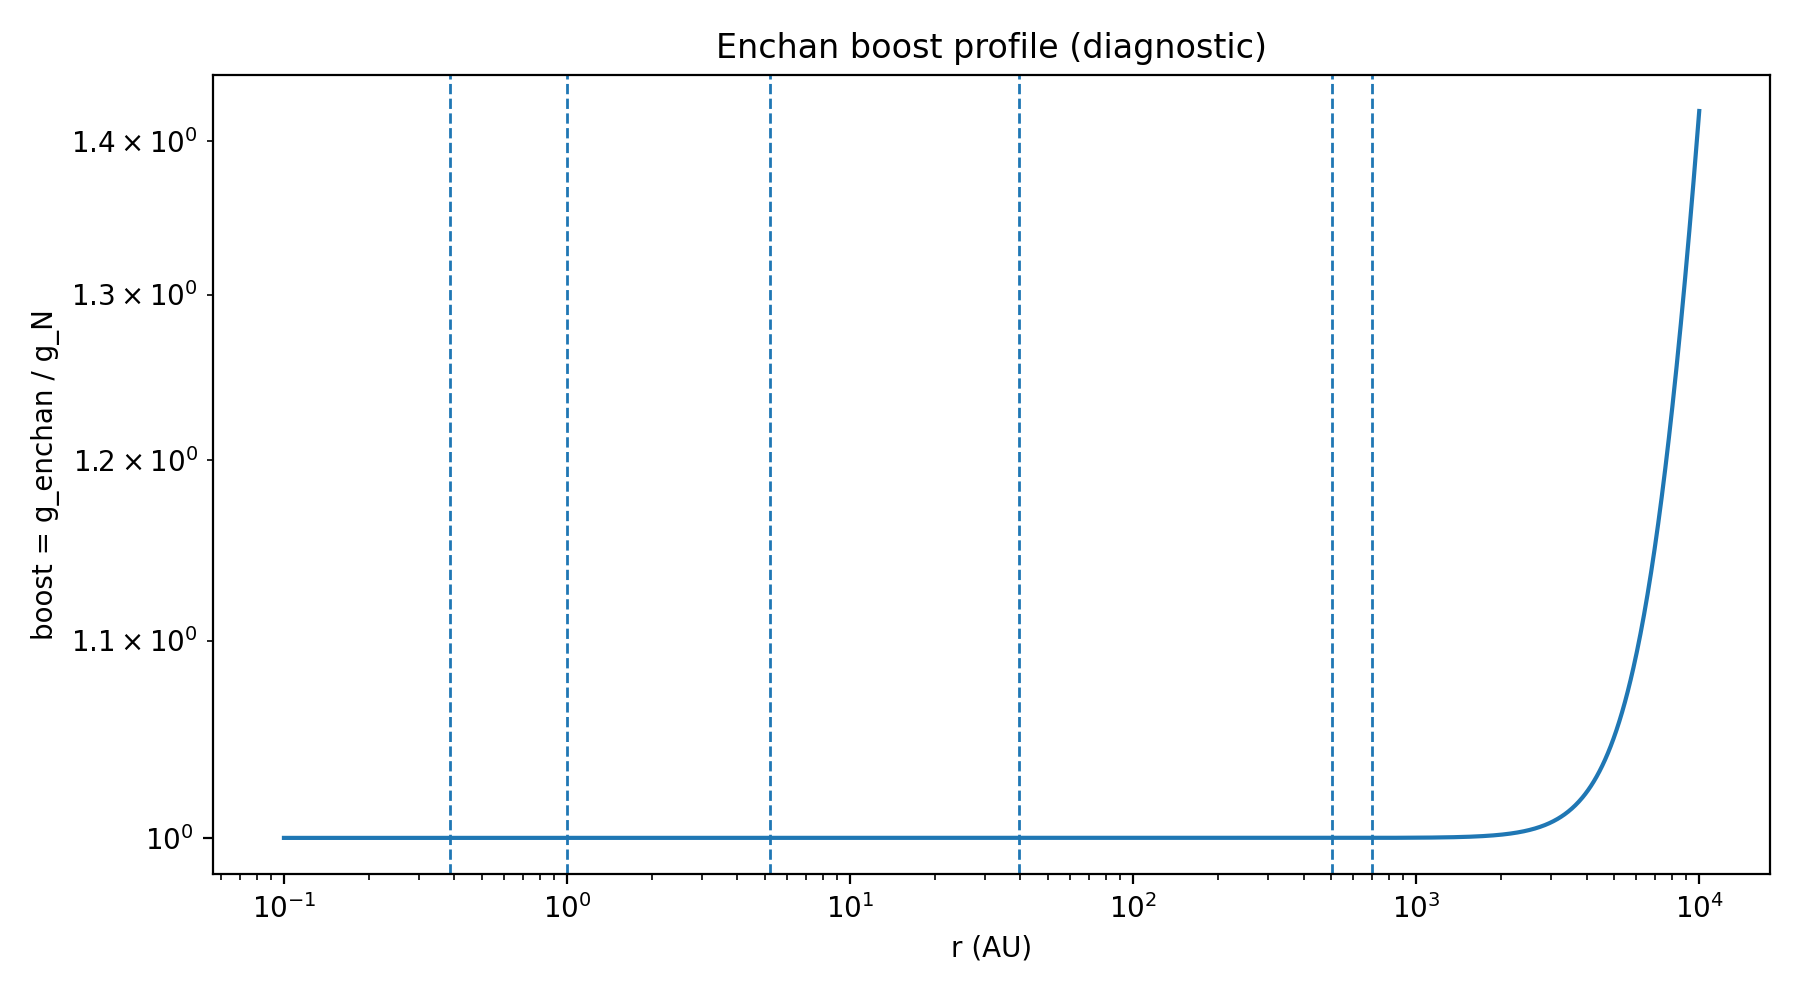
\includegraphics[width=0.8\textwidth]{figures/enchan_solar_system_delta_accel_boost.png}
    \caption{Diagnostic boost profile $g_{\rm Enchan}/g_N$ under high-acceleration screening. The profile remains close to unity throughout the planetary regime and rises only toward far outer Solar-System radii. This is a consistency diagnostic, not a full ephemeris fit.}
    \label{fig:solar_boost}
\end{figure}

\begin{figure}[h]
    \centering
    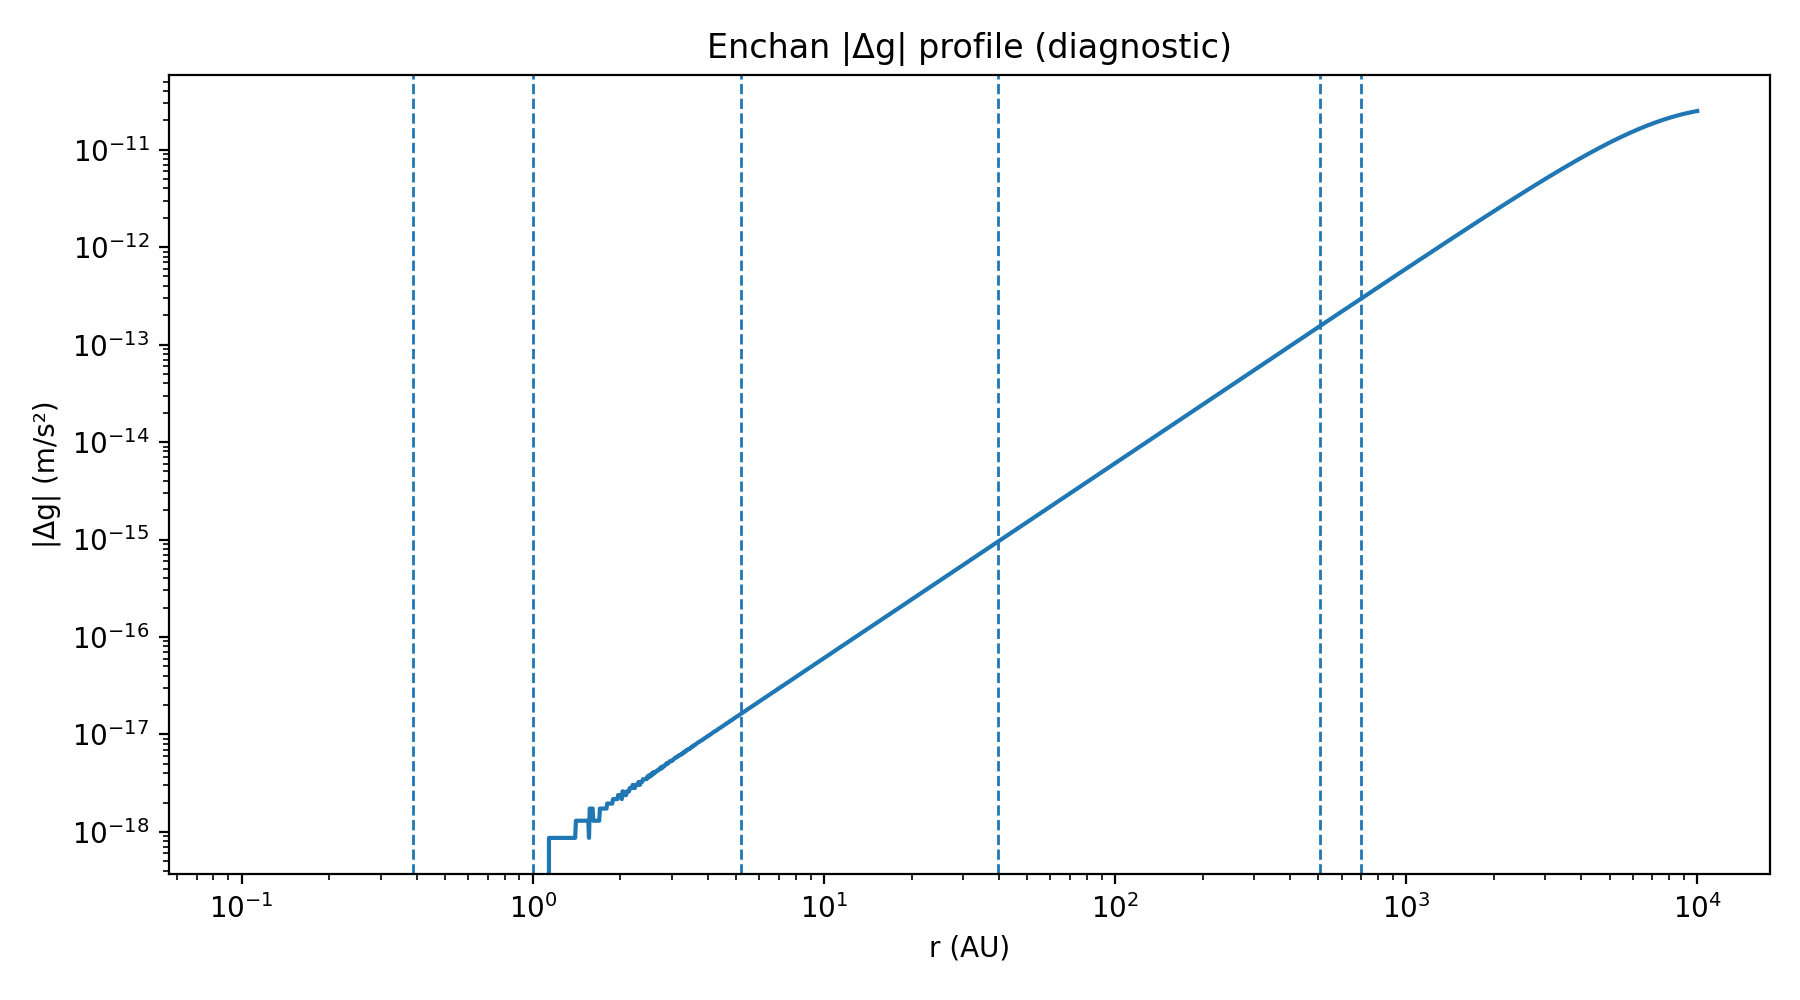
\includegraphics[width=0.8\textwidth]{figures/enchan_solar_system_delta_accel_delta_g.png}
    \caption{Diagnostic residual acceleration $|\Delta g|=|g_{\rm Enchan}-g_N|$. The residual remains strongly suppressed in high-acceleration inner regions, supporting recovery of the Newtonian limit within the tested profile.}
    \label{fig:solar_delta_g}
\end{figure}

This result should be treated as a consistency check rather than an observational claim. A full comparison with Solar-System ephemerides, ranging data, and post-Newtonian constraints remains outside the scope of the present paper.

\clearpage

\section{Translation to Discrete Graph Dynamics}

Scale-free graphs provide a discrete testbed for the same stabilization principle. In such graphs, high-degree hub nodes represent localized over-concentrations of interaction intensity. If all interactions are aggregated linearly, these hubs can dominate the global landscape and force premature convergence.

NP-hard problems like Max-Cut can be formulated as finding the ground state of an Ising Hamiltonian. In standard continuous-variable models, discrete spins $s_i \in \{-1, +1\}$ are relaxed into continuous variables $x_i \in [-1, +1]$. The state evolution is driven by the local field interaction:
\begin{equation}
H_i = \sum_j W_{ij} x_j
\end{equation}
where $W_{ij}$ is the adjacency matrix.

\subsection{Hub-Induced Over-Curvature}

Under linear coupling, the local field $H_i$ around a high-degree hub grows disproportionately. This creates topological over-curvature: a localized region of excessive influence that distorts the relaxation landscape. In practical optimization, this appears as hub-induced collapse, where the system rapidly stabilizes into shallow local minima.

\subsection{Deep-Potential Pinning and the Discrete Screening Map}

A rigorous reader might observe a mathematical leap: the continuous field formulation (Eq.~\ref{eq:FieldEqMu}) defines non-linear saturation based on the local gradient ($\nabla S$), yet the discrete mapping applies the screening function to the aggregate local field $H_i$, not the individual edge differences. Why does the saturation apply to the node's total input?

The high-acceleration diagnostic above suggests a useful interpretation. In deep-potential environments, the effective anomalous response can be strongly suppressed and the local dynamics approach the Newtonian limit within the tested profile. This indicates that finite tension may manifest not only as a limit on local gradients, but also as environmental suppression within regions of large background acceleration or potential depth.

In this interpretation, the local environment pins the effective rules of interaction. The discrete graph analogue is a high-degree hub: its aggregate local field $H_i$ represents not merely a force vector, but the depth of the node's effective interaction environment. Applying screening to $H_i$ therefore implements a discrete version of deep-potential pinning.

The mapping should be read as a computational analogue rather than a strict mathematical isomorphism. The continuous quantity $\nabla S$ and the discrete aggregate field $H_i$ are not asserted to be identical mathematical objects. Rather, both play the role of local concentration measures that can dominate the global relaxation process if left unscreened.

\subsection{Finite-Tension Screening on Graphs}

In a discrete scale-free graph, a high-degree hub node is the topological analogue of a deep gravitational potential well. The aggregate local field $H_i$ represents the depth of this effective potential. Therefore, the Enchan Field screening principle is translated into graph dynamics by replacing unrestricted linear aggregation with a finite-tension response applied to the hub's total environment:
\begin{equation}
\mu_i(H_i) \approx \frac{1}{1 + (|H_i|/a_0)^\alpha}.
\end{equation}
The effective local influence is then regularized by $\mu_i(H_i)$, preventing high-degree hubs from overwhelming the global relaxation.

As the magnitude of the local field $H_i$ exceeds $a_0$, the effective coupling is dampened. By treating $H_i$ as an environmental potential depth rather than a simple aggregated force vector, this operation is interpreted as the discrete expression of the deep-potential pinning principle: excessive local concentration must be regularized for global stabilization to emerge.

\subsection{Enchan Cosmic as Computational Realization}

Enchan Cosmic is the computational engine that realizes this field principle in discrete graph optimization. It should be understood as an implementation of Enchan Field relaxation, not as the source of the theory itself. The solver exposes how non-linear stabilization behaves when applied to large-scale topological structures.

\clearpage

\section{Empirical Observations}

The resulting computational engine was tested on both synthetic and real-world scale-free graphs to observe its relaxation behavior.

The purpose of this section is not to establish Enchan Cosmic as a state-of-the-art Max-Cut solver, but to show that the same finite-tension stabilization principle can be realized as a deterministic relaxation process on large discrete topologies.

\subsection{Observation on Scale-Free Networks}
Optimization tests were performed on a synthetic scale-free network (Barab\'{a}si--Albert model, 100,000 nodes) and a real-world web graph (SNAP Web-Google, 875,713 nodes).
\begin{itemize}
    \item When strictly linear coupling was applied, the system exhibited premature convergence characteristic of hub-induced collapse.
    \item Upon introducing the non-linear screening function $\mu_i(H_i)$, the system avoided early stabilization in shallow minima and converged to higher cut ratios.
\end{itemize}

\subsection{Scale Invariance and Stability}
Execution on a 1-million node random sparse graph completed in 2.56 seconds using standard CPU hardware. The system remained mathematically stable without manual hyperparameter grid-search, due to the dynamic derivation of Courant--Friedrichs--Lewy (CFL) stability limits scaled against the field parameters.

\subsection{Benchmark Audit Snapshots}

The following audit snapshots document representative benchmark runs used as computational diagnostics. They are included as reproducibility artifacts rather than as standalone proof of optimality.

\begin{figure}[h]
    \centering
    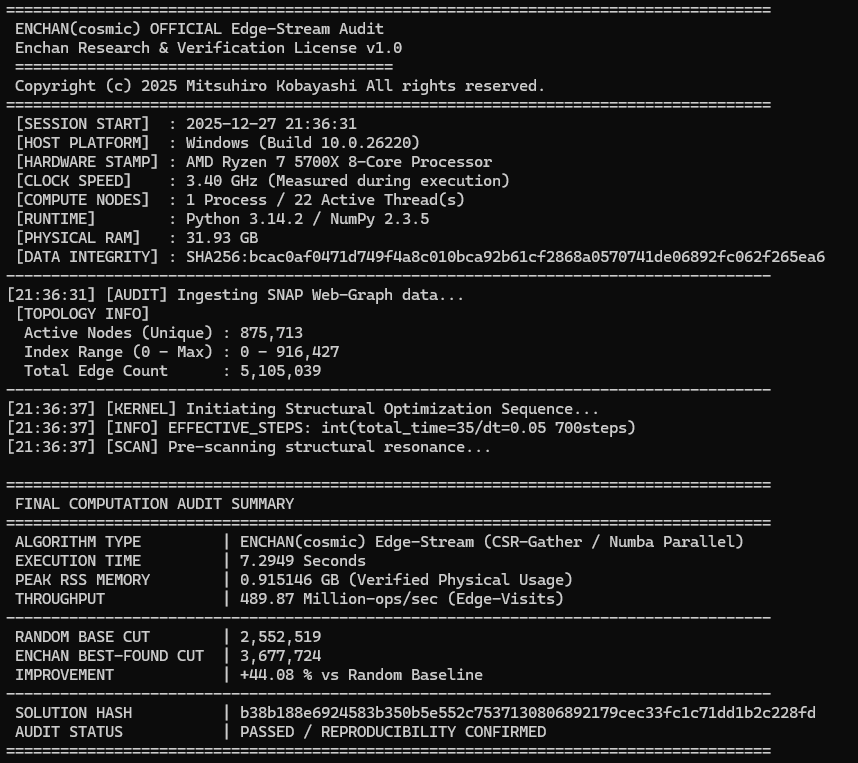
\includegraphics[width=0.92\textwidth]{figures/enchan_web_google_audit.png}
    \caption{Representative SNAP Web-Google audit snapshot for Enchan(cosmic) Edge-Stream optimization. The run reports 875,713 active nodes, 5,105,039 edges, a best-found cut of 3,677,724, and a +44.08\% improvement against the random baseline in this diagnostic protocol. The snapshot should be read as an audit artifact for the reported implementation and data integrity conditions.}
    \label{fig:web_google_audit}
\end{figure}

\begin{figure}[h]
    \centering
    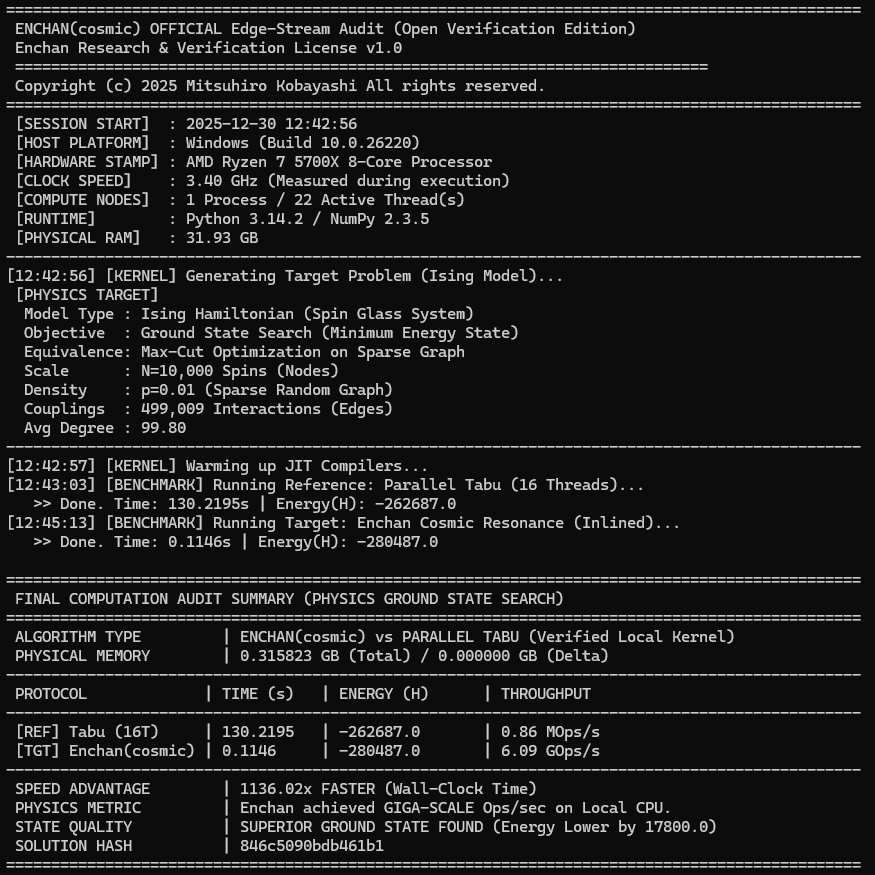
\includegraphics[width=0.92\textwidth]{figures/enchan_ising_tabu_comparison.png}
    \caption{Representative 10,000-spin Ising / sparse Max-Cut audit snapshot comparing Enchan(cosmic) with a parallel Tabu reference on the same local CPU environment. The snapshot reports the wall-clock timing, energy values, and solution hash for this benchmark instance, and is included as a computational diagnostic rather than a general performance theorem.}
    \label{fig:ising_tabu_audit}
\end{figure}

\clearpage

\subsection{Implementation Availability}

While the static snapshots provided above confirm the computational stability and diagnostic behavior of the Enchan Field principle on discrete topologies, the live implementation of the solver is maintained as an accessible service. Readers interested in practical optimization, dynamic verification, or the specific computational architecture of the solver are referred to the Enchan Cosmic Public API and its accompanying technical whitepaper:
\begin{center}
    \url{https://github.com/EnchanTheory/Enchan-Web-OS}
\end{center}

\clearpage

\section{Scope and Relation to Existing Frameworks}

\subsection{Three-Layer Structure of the Proposal}

The present paper should be read as a three-layer framework. The first layer is the field-theoretic layer: finite field tension is represented through a non-linear kinetic response. The second layer is the correspondence layer: the transition from $\nabla S$ to $H_i$ is treated as a role-based computational analogy, not as a strict mathematical identification. The third layer is the implementation layer: Enchan Cosmic is one discrete computational realization of the stabilization principle.

This layered interpretation limits the scope of the claim. The paper does not assert that the continuous field equation and the discrete graph update rule are identical mathematical systems. It asserts that both can be organized around the same finite-tension stabilization principle.

\subsection{Relation to k-essence and Modified-Gravity Models}

The non-linear kinetic structure used here is mathematically related to k-essence-type effective field theories and to broader scalar-field approaches in modified gravity. The novelty claimed in this paper is not the use of a non-linear kinetic term by itself. Rather, the proposed contribution is the interpretation of such a term as a finite-tension stabilization vessel, together with its translation into deterministic relaxation dynamics on discrete graph topologies.

This paper does not claim to supersede existing k-essence, MOND-like, TeVeS-like, or scalar-field modified-gravity models. It instead proposes an effective framework in which finite-tension screening, geometric stabilization, and discrete optimization can be discussed using a shared relaxation language. A detailed comparative analysis against existing relativistic and nonrelativistic modified-dynamics theories is outside the scope of the present v1.0.0 formulation.

\subsection{Field-First Development and Computational Realization}

The computational implementation emerged after the initial Enchan Field notes had already been written and publicly released \cite{KobayashiFieldNotes}. Its original purpose was not to build a graph solver, but to test whether the field equations and relaxation principles could be instantiated as a working computational process.

The later observation that this process behaved as a deterministic graph-optimization engine is therefore treated as a consequence of the field formulation, not as the premise from which the field formulation was derived. Thus, Enchan Cosmic should be understood as a computational realization and diagnostic extension of the prior field framework.

\clearpage

\section{Discussion}

\subsection{Optimization as Geometric Relaxation}

Optimization on a graph is typically viewed as a series of discrete arithmetic operations. The Enchan Field suggests a different interpretation: optimization can be understood as relaxation within a continuous interaction medium. The binary solution emerges not only from search, but from the formation of stable phase boundaries under field constraints.

In this context, the term \emph{deterministic} refers to the strictly reproducible evolution of the system state as defined by its effective field equations. Unlike standard stochastic optimization methods (e.g., simulated annealing) that rely on random thermal noise to escape local minima, the Enchan Field avoids premature convergence through the deterministic regularization of its non-linear tension.

In this view, candidate cut surfaces correspond to phase boundaries formed during relaxation. They should not yet be claimed to map exactly to globally optimal cuts in all cases. Rather, they represent stable separations induced by the geometry of the interaction field.

\subsection{Relation to Modified-Dynamics Approaches}

The Enchan Field has a retrospective structural similarity to modified-dynamics approaches in the limited sense that both question unrestricted linear extrapolation across all scales. This relation is not one of derivation, but of structural analogy.

In particular, Modified Newtonian Dynamics (MOND) modifies the low-acceleration regime, whereas the graph-dynamical Enchan Field introduces saturation in the high-local-field regime. The shared idea is not the direction of correction, but the existence of a characteristic scale at which the effective interaction law changes.

Thus, the Enchan Field should be understood primarily as a finite-tension stabilization framework. Its screening response is closer to regularization of excessive concentration than to weak-field enhancement.

\subsection{Relation to earlier field-note formulations}

The present paper generalizes earlier Enchan Field notes that emphasized topological defects, asymptotic $1/r^2$ energy-density profiles, and flat rotation signatures. Those notes remain useful as phenomenological and historical precursors. However, the present formulation changes the theoretical center of gravity: the primary object is no longer a defect sector alone, but a finite-tension geometric stabilization field whose non-linear kinetic response can generate screening, regularization, and phase-boundary formation across both continuous and discrete systems.

\subsection{Limitations}

The current formulation is an effective field model and does not yet provide a complete fundamental theory of spacetime, gravity, or cosmology. The astrophysical section demonstrates a plausible stabilization signature, while the graph section demonstrates a computational realization of the same principle. The Solar-System high-acceleration calculation is included only as a diagnostic extrapolation; it is not a substitute for full ephemeris fitting or precision-gravity constraints. Further work is required to derive stronger observational predictions, establish uniqueness conditions, and compare against broader classes of optimization algorithms. The benchmark audit snapshots document representative local runs, but a fuller reproducibility package should include complete hardware metadata, edge-list provenance, implementation language and version, stopping criteria, cut-ratio definitions, and deterministic hash-confirmation procedures.

\section{Conclusion}

We introduced the Enchan Field as an effective field framework for geometric stabilization. Its core idea is that coherent structures can arise from the relaxation of an interaction medium with finite field tension. When local concentration exceeds a characteristic scale, the field responds non-linearly, regularizing excessive deformation and preventing collapse.

This principle provides a common language for two domains that are usually treated separately. In astrophysical interpretation, it offers a geometric route to large-scale stabilization signatures such as approximately flat rotation profiles. In discrete graph dynamics, it explains why non-linear screening can suppress hub-induced collapse in scale-free networks.

The Enchan Field is therefore proposed as a unifying formalism for stabilization phenomena across continuous geometry and discrete topology. Enchan Cosmic is one computational realization of this principle, demonstrating that deterministic optimization can be interpreted as geometric relaxation within a finite-tension interaction field.

\clearpage

\bibliographystyle{plain}
\begin{thebibliography}{9}

\bibitem{KobayashiFieldNotes}
M.~Kobayashi,
\newblock Enchan Field Notes.
\newblock Public repository, \url{https://github.com/EnchanTheory/Enchan-Field-Notes}, 2025--2026.

\bibitem{Milgrom1983}
M.~Milgrom,
\newblock A modification of the Newtonian dynamics as a possible alternative to the hidden mass hypothesis.
\newblock {\em The Astrophysical Journal}, 270:365-370, 1983.

\bibitem{Goto2019}
H.~Goto et al.,
\newblock Combinatorial optimization by simulating adiabatic bifurcations in nonlinear Hamiltonian systems.
\newblock {\em Science Advances}, 5(4):eaav2372, 2019.

\bibitem{Leskovec2009}
J.~Leskovec et al.,
\newblock Community Structure in Large Networks: Natural Cluster Sizes and the Absence of Large Well-Defined Clusters.
\newblock {\em Internet Mathematics}, 6(1):29-123, 2009.

\end{thebibliography}

\end{document}